\documentclass{article}
\usepackage{ctex}
\usepackage{graphicx}
\usepackage{amsmath}
\usepackage{indentfirst}
\usepackage{titlesec}
\usepackage{setspace}
\usepackage{subfigure}
\usepackage{caption}
\usepackage{float}
\usepackage{booktabs}
\usepackage{geometry}
\usepackage{multirow}
\usepackage{hyperref}
\hypersetup{
	colorlinks=true,
	linkcolor=blue,
	filecolor=magenta,      
	urlcolor=cyan,
	pdftitle={Overleaf Example},
	pdfpagemode=FullScreen,
}
\geometry{left=1.2cm,right=1.2cm,top=2cm,bottom=2cm}
\title{\songti \zihao{2}\bfseries HW8第13题Metropolis-Hasting算法}
\titleformat*{\section}{\songti\zihao{4}\bfseries}
\titleformat*{\subsection}{\songti\zihao{5}\bfseries}
\renewcommand\thesection{\arabic{section}}
\author{王启骅 PB20020580}
\begin{document}
	\maketitle
	\section{题目}
	用Metropolis-Hasting抽样方法计算积分:
	\begin{equation}
		I=\int_{0}^{\infty}(x-\alpha\beta)^2f(x)dx=\alpha\beta^2
		\nonumber
	\end{equation}
其中$ f(x)=\frac{1}{\beta\Gamma(x)}(\frac{x}{\beta})^{\alpha-1}\exp(-x/\beta) $,设积分权重函数为p(x)=f(x)和$  p(x)=(x-\alpha\beta)^2f(x) $


给定参数$ \alpha,\beta $ ,并用不同的$ \gamma $ 值,分别计算积分,讨论计算精度和效率。
	
	\section{算法原理}
首先对于p(x)=f(x)的情况,取
\begin{equation}
	T(x\rightarrow x')=\frac{1}{\gamma}\exp(x'/\gamma)
\end{equation}
可以产生抽样$ x'=-\gamma \ln(R) $,其中R为[0,1]的均匀分布。
\begin{equation}
	r=\big(\frac{x'}{x_i}\big)^{\alpha-1}\exp(-(x'-x_i)/\beta)\exp((x'-x_i)/\gamma)
\end{equation}
对于试探步的取舍情况为
\begin{equation}
	x_{i+1}=
	\begin{cases}
		x'&\text{if R<min(1,r)}\\
		x_i&\text{if R>min(1,r)}
	\end{cases}
\end{equation}
最后可计算积分值为
\begin{equation}
	I=\frac{1}{N-m}\sum_{i=m+1}^{N}(x_i-\alpha\beta)^2
\end{equation}

对于取$ p(x)=(x-\alpha\beta)^2f(x) $的情况,相类似以同样的抽样方式
\begin{equation}
	T(x\rightarrow x')=\frac{1}{\gamma}\exp(x'/\gamma)
\end{equation}
可以产生抽样$ x'=-\gamma \ln(R) $,其中R为[0,1]的均匀分布。
\begin{equation}
	r=\big(\frac{x'-\alpha\beta}{x_i-\alpha\beta}\big)^2\big(\frac{x'}{x_i}\big)^{\alpha-1}\exp(-(x'-x_i)/\beta)\exp((x'-x_i)/\gamma)
\end{equation}
对于试探步的取舍情况为
\begin{equation}
	x_{i+1}=
	\begin{cases}
		x'&\text{if R<min(1,r)}\\
		x_i&\text{if R>min(1,r)}
	\end{cases}
\end{equation}
由于初始$ p(x)=(x-\alpha\beta)^2f(x) $未进行归一化,需要乘以归一化因子$ \alpha\beta^2 $可计算积分值为
\begin{equation}
	I=\frac{1}{N-m}\sum_{i=m+1}^{N}\alpha\beta^2
\end{equation}
其实由此可以见到,该积分对于每次抽样后所取的函数值均为1,实际上积分得到的是精确结果。对于模拟该抽样方法时,由于需要提前将函数归一化,需要已知该积分的准确值,归一化后才能进行计算,所以可见该抽样方法对于分析积分的误差及效率没有太大意义。
	\section{结果}
	\subsection{计算结果精度}
	这部分对应程序HW8\_13\_Metropolis.f90
	
	
	这里讨论$\alpha$=2,$\beta$=1的情况。首先产生$ n=10^6 $个点的Markov链,并且取前$ m=\frac{n}{10} $的点舍弃作为热化阶段,取了$ \gamma=0.1-50 $,以0.1为步长,计算结果的绝对误差
	\begin{equation}
		|I-\alpha\beta^2|
	\end{equation}
与抽样效率
	\begin{figure}[!h]
	
	\centering
	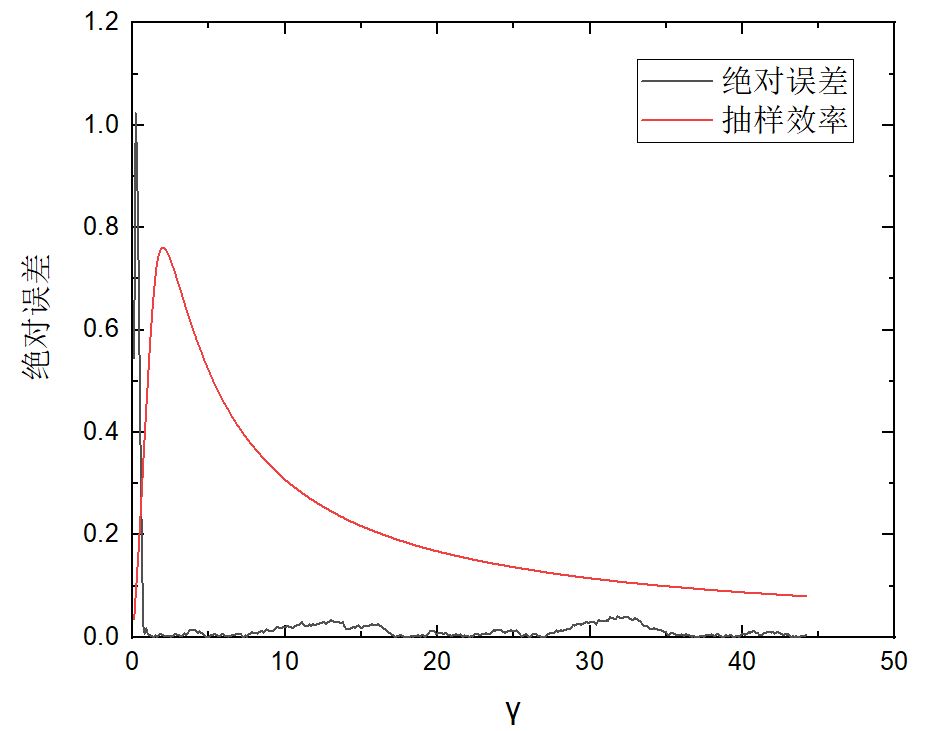
\includegraphics[scale=0.6]{error_eff_1}
	\captionsetup{font={small},labelfont=bf}
	\caption{\heiti\zihao{-5}计算结果}
	\label{fig:1}
\end{figure}
由图\ref{fig:1}分析大致趋势可以得到在$ \gamma=0-1 $的区间绝对误差处在剧烈的振荡,之后$\gamma$=1处迅速趋近于0,并在之后的区间中在0附近上下振荡,但误差不超过$ 10^{-1} $。并且抽样效率先上升,再下降,在$\gamma$=2时取到最大值0.75 。


	\begin{figure}[!h]
	
	\centering
	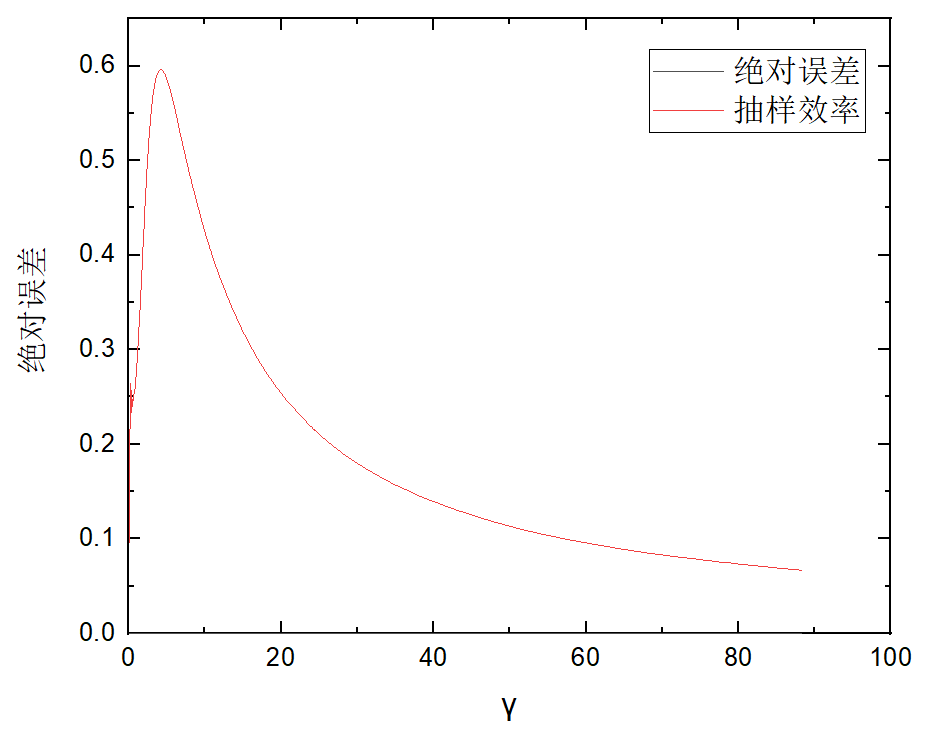
\includegraphics[scale=0.5]{error_p2}
	\captionsetup{font={small},labelfont=bf}
	\caption{\heiti\zihao{-5}$ p(x)= (x-\alpha\beta)^2f(x)$下计算结果}
	\label{fig:2}
\end{figure}
对于p(x)=$ (x-\alpha\beta)^2f(x) $的情况,相似的方法作图如图\ref{fig:2},根据图可见其绝对误差恒等于0,txt文件中得到的绝对误差数据在$ 10^{-12} $,来源于计算机本身误差。同样抽样效率也先上升,然后趋于0 。由此可见对于该抽样方法的讨论没有太大意义。
\subsection{计算效率}
这部分对应程序HW8\_13\_Metro\_eff.f90


接下来讨论计算效率,分析计算结果的绝对误差随Metropolis-Hasting方法取点数的关系。由于第二种抽样函数下不存在误差,这里只分析第一种抽样函数进行分析。这里取了从$ n=10-10^7 $个点,取前$ m=\frac{n}{10} $的点舍弃作为热化阶段。并根据以上实验的结果图\ref{fig:1},再$ \gamma=3,\ 18,\ 27$附近的较大区间内绝对误差始终处于较小的趋近于0的范围,所以这里设定$ \gamma=3,\ 18,\ 27 $,绘制出绝对误差随取点数的变化图\ref{fig:3},
	\begin{figure}[!h]
	
	\centering
	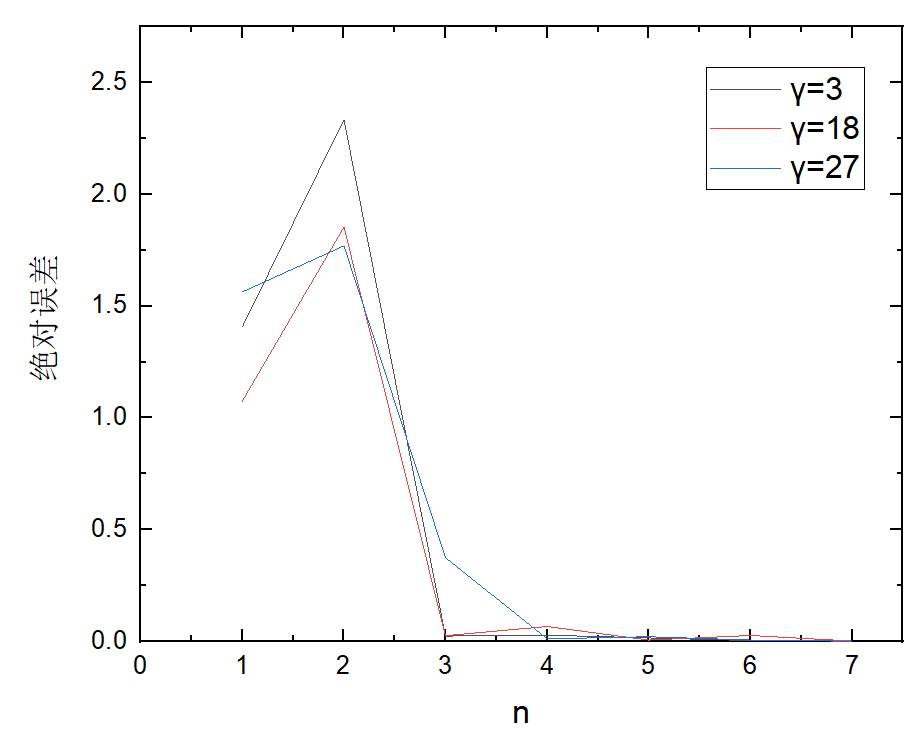
\includegraphics[scale=0.6]{error_n}
	\captionsetup{font={small},labelfont=bf}
	\caption{\heiti\zihao{-5}计算效率}
	\label{fig:3}
\end{figure}
分析图可以得到随着Markov链随机行走的步数量级增加,绝对误差首先在$ 10-10^2 $区间先上升,之后在$ n<10^4 $阶段迅速下降,最后逐渐趋近于0,再进一步提高行走步数时误差基本不再变化。
	\section{结论}
	本次模拟通过Metropolis-Hasting方法模拟积分,讨论了积分精确度和抽样效率,计算效率的关系,寻找到了使积分精度达到最高的$ \gamma $值。根据计算效率的测试结果,可以得到在所取步数量级大于$ 10^4 $后,计算精度基本不变,因此为了计算时间和内存的考虑不需要将计算步数取到非常大。
\end{document}